\documentclass[main.tex]{subfiles}

\begin{document}

\chapter{Problem 1.1 - Penalty Method}

\section{Problem Description}

In this problem, goal was to find the minimum of the objective, constrained, binomial function 

\begin{equation}
f(x_1,x_2) = (x_1 - 1)^2 + 2*(x_2 - 2)^2
\end{equation}

that is subject to the inequality constraint function

\begin{equation}
g(x_1,x_2) = x_1^2 + x_2^2 - 1 \leq 0.
\end{equation}

Problem may be presented graphically by plot in 3 dimensions as below:

\begin{figure}[h]
\label{fig:solution}
\centering
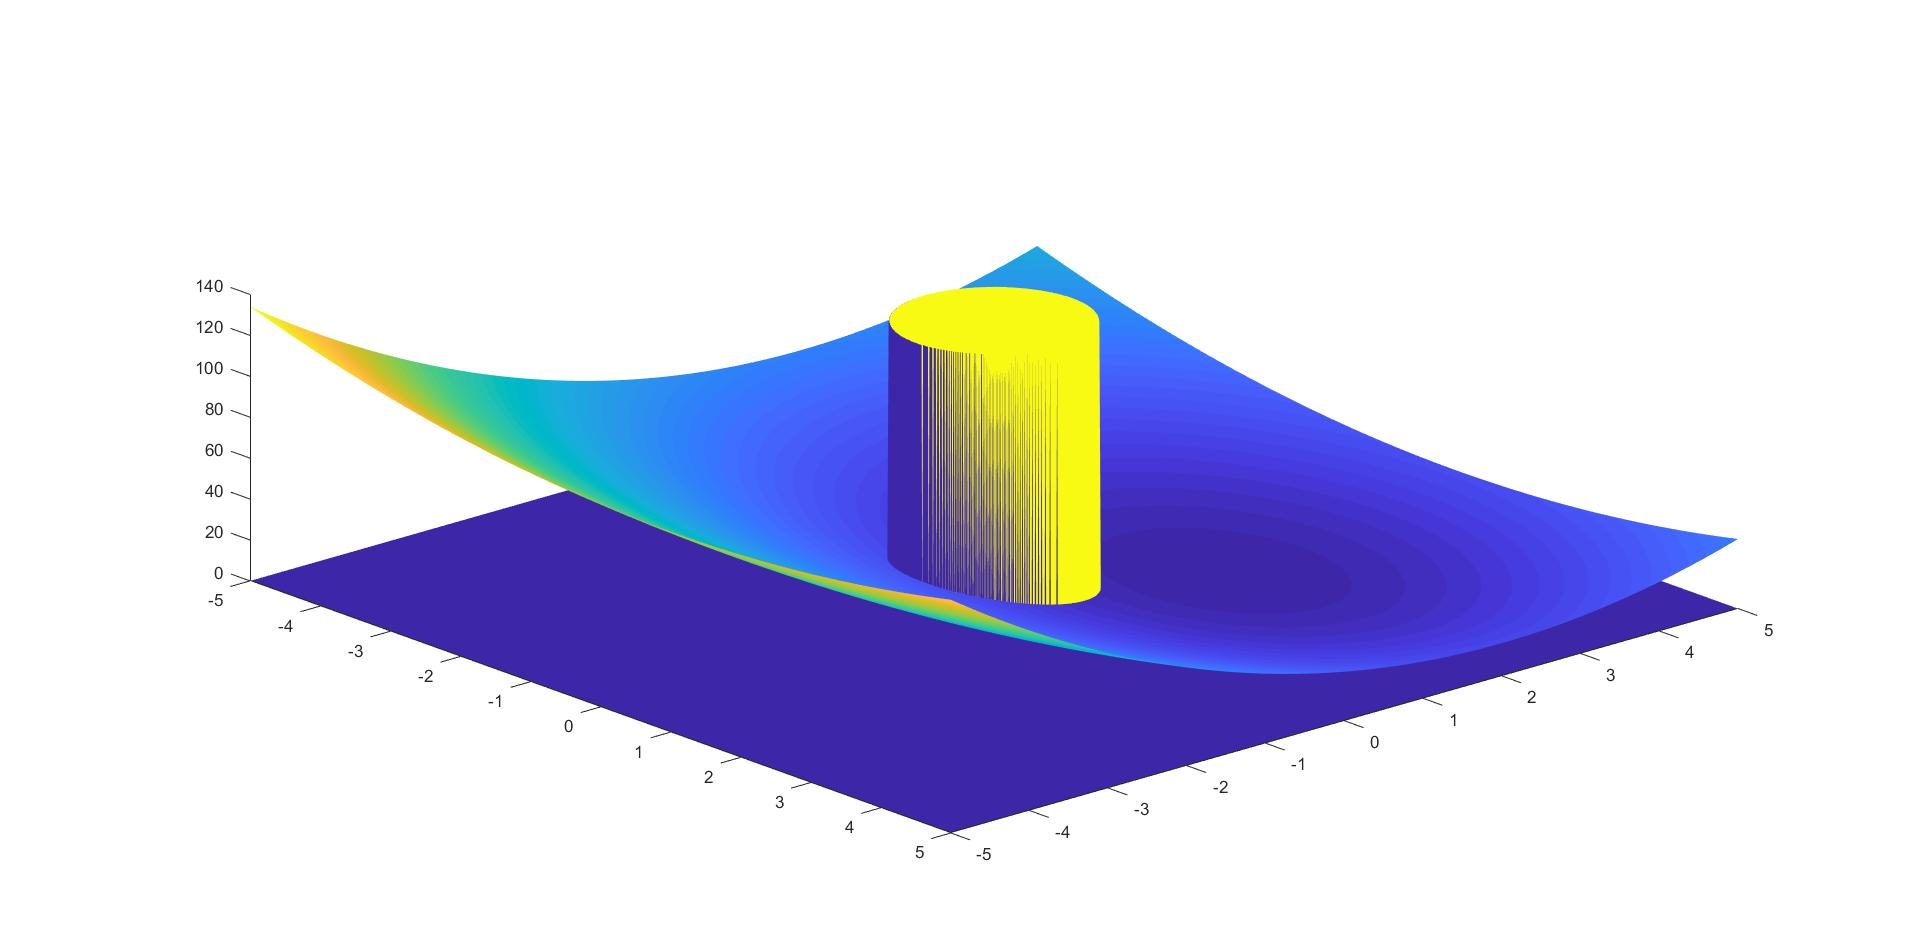
\includegraphics[width=\textwidth]{PenaltyMethod/PenaltyMethod_constrained_fx.jpg}
\caption{Objective Function with constraints.}
\end{figure}

and with vertical projection on the plane $(x_1, x_2)$

\begin{figure}[h]
\label{fig:solution}
\centering
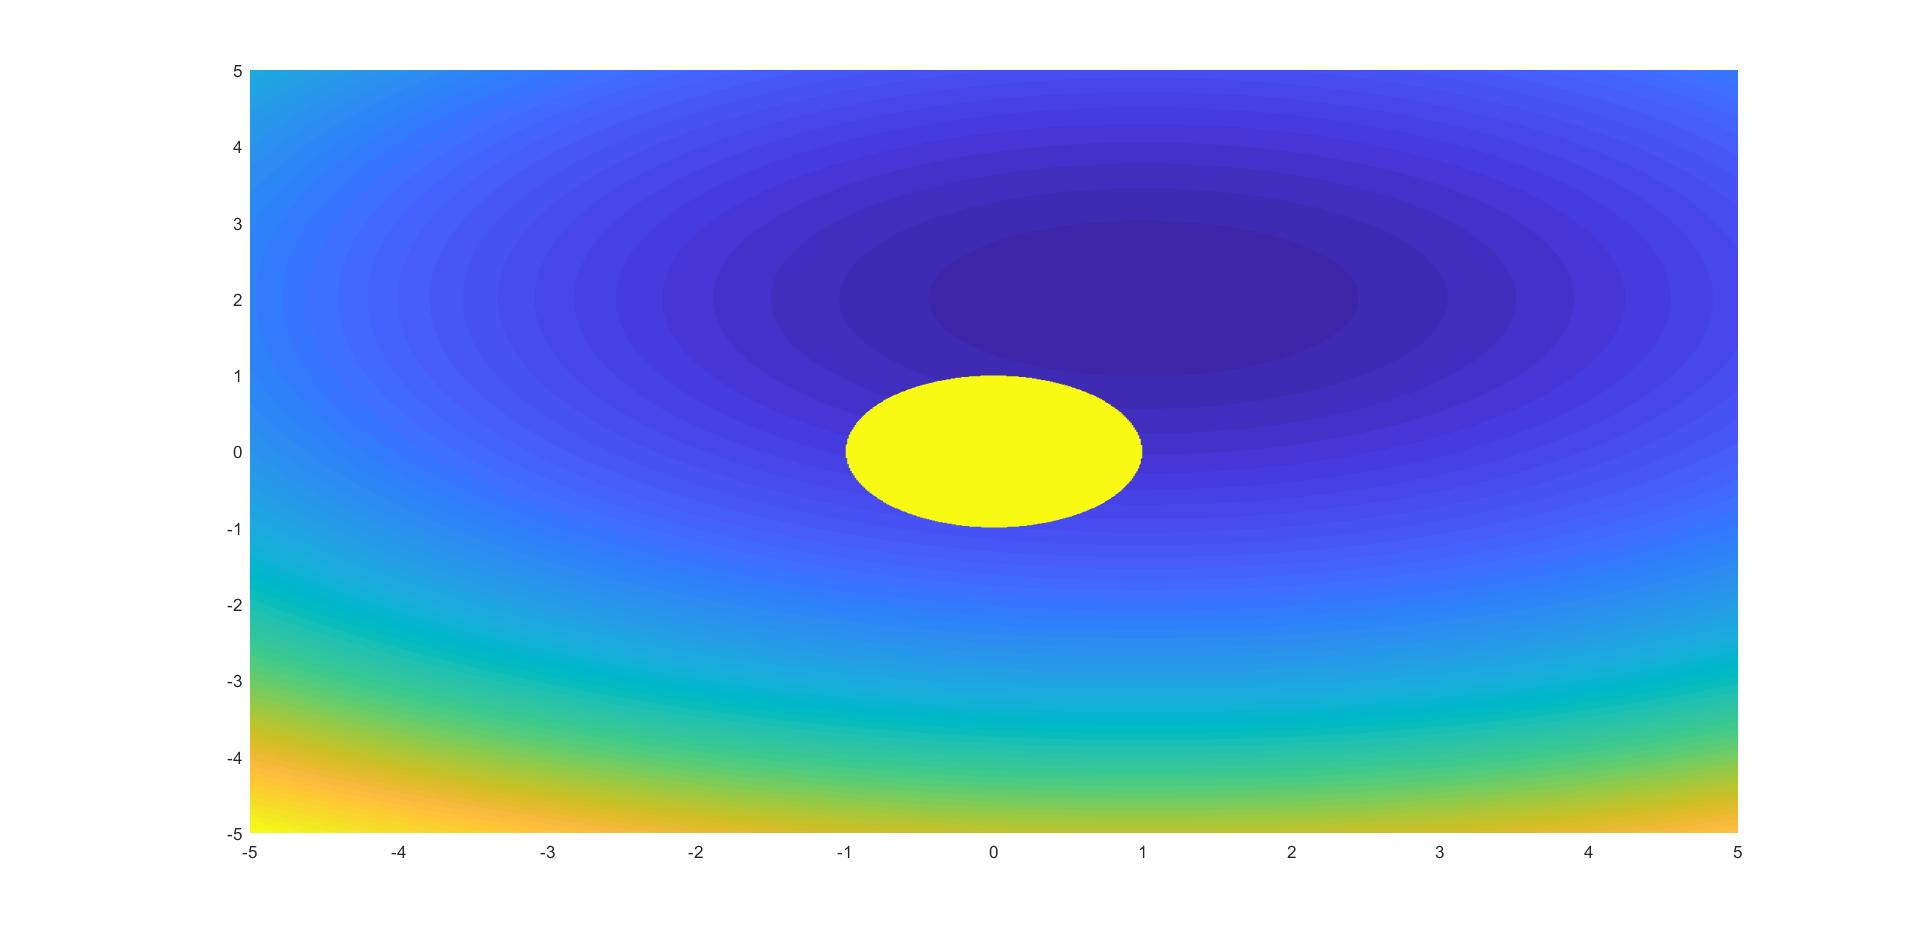
\includegraphics[width=\textwidth]{PenaltyMethod/PenaltyMethod_constrained_fx_view(0,90)_.jpg}
\caption{Objective Function with constraints with vertical view.}
\end{figure}


Following "Home Problems 1 Instruction" this task include steps that are listed below as copy:

\begin{enumerate}
    \item Define (and specify clearly, in your report, as a function of $x_1$, $x_2$, and $\mu$) the function $f_p(x;\mu)$, consisting of the sum of $f(x_1,x_2)$ and the penalty term $p(x;\mu)$.
    \item Compute (analytically) the gradient $\nabla{f_p(x;\mu)}$, and include it in your report.
    \item Find and report the unconstrained minimum (i.e. for $\mu = 0$) of the function. This point will be used as the starting point for gradient descent.
    \item Write a Matlab program for solving the unconstrained problem of finding the minimum of $f_p(x;\mu)$ using the method of gradient descent. 
    \begin{enumerate}
        \item A main file PenaltyMethod.m (that calls the other functions, generates and prints output etc. etc.). This program should not require any input, i.e. to run it, one should only need to write PenaltyMethod in Matlab, without having to specify any input parameters. The necessary parameters may be hardcoded in PenaltyMethod.m; see also below. 
        \item A function (in a separate file, GradientDescent.m), which takes the starting point $\vec{x}_{(0)}$ (as a vector with two elements), the value of $\mu$, the step length (for gradient descent) $\eta$, and a threshold T (see below) as input, and carries out gradient descent until the modulus of the gradient, $|\nabla{f_p(\vec{x};\mu)}|$, drops below the threshold T. Use the unconstrained minimum at the starting point; see above. 
        \item A function Gradient (in a separate file, Gradient.m) which takes as input the values of $x_1, x_2$, and $\mu$, and returns the gradient of $f_p(\vec{x};\mu)$ (a vector with two elements). Note: You may hardcode the gradient in this method, i.e. you do not need to write a general method for finding the gradient. However, your method should make use of the analytical gradient, computed in Step 2 above. You should not use a numerical approximation of the gradient.
    \end{enumerate}
    \item Run the program for a suitable sequence of $\mu$ values (which you may hard-code in PenaltyMethod.m). Select a suitable (small) value for the step length $\eta$, and specify it clearly, along with the sequence of $\mu$ values, in your report. Example of suitable parameter values: $\eta = 0.0001$, $T = 10e-1$, sequence of $\mu$ values: 1, 10, 100, 1000.
    
\end{enumerate}

Program in Matlab is not required to be reported, so only instruction of "how to" run it will be attached and necessary results with graphic output. Next sections will be describing steps used for solving this task.

\newpage 
\section{Step 1}
Using the penalty method (pp. 30-33 in the course book) we rewrite problem as unconstrained objective function

\begin{equation}
f_p( x_1, x_2, \mu ) = f(x_1,x_2) + p(x_1,x_2,\mu)
\end{equation}

where $f(x_1, x_2)$ is constrained objective function and 

\begin{equation}
p(x_1,x_2,\mu) = \mu*max\{0, x_1^2 + x_2^2 -1\}^2
\end{equation}

is penalty term (function), what could be rewritten as

\begin{equation}
p(x_1,x_2,\mu) = \mu*\left \{
  \begin{tabular}{lrr}
  $a(x_1,x_2)^2$ & if & $a(x_1,x_2) >= 0$\\
  $0$ & & otherwise\\
  \end{tabular}
\right
\end{equation}

and where

\begin{equation}
a(x_1, x_2) = x_1^2 + x_2^2 -1.
\end{equation}

\newpage
\section{Step 2}

Solution with penalty method algorithm included gradient descent, where gradient is of unconstrained objective function and it has form

\begin{equation}
\nabla{f_p(x_1,x_2,\mu)} = \nabla{f(x_1,x_2)} + \nabla{p(x_1,x_2,\mu)}
\end{equation}

Gradient of objective function

\begin{equation}
    \nabla{f(x_1,x_2)} = \left(
    \frac{\partial{f(x_1,x_2)}}{\partial{x_1}}, \frac{\partial{f(x_1,x_2)}}{\partial{x_2}}
    \right)  
\end{equation}

contains partial derivatives over variables $x_1$, derived as

\begin{equation}
     \frac{\partial{f(x_1,x_2)}}{\partial{x_1}} = 2*(x_1-1)
\end{equation}

and over $x_2$, derived as

\begin{equation}
 \frac{\partial{f(x_1,x_2)}}{\partial{x_2}} = 4*(x_2-2).
\end{equation}

Also, gradient of penalty function is of a form

\begin{equation}
    \nabla{p(x_1,x_2,\mu)} = \mu*\left(
    \frac{\partial{p(x_1,x_2,\mu)}}{\partial{x_1}}, \frac{\partial{p(x_1,x_2,\mu)}}{\partial{x_2}}
    \right)  
\end{equation}

for which partial derivatives over variables $x_1$ and $x_2$ are derived ($\mu$ is treated as constant parameter, not to be derived for) respectively as 

\begin{equation}
     \frac{\partial{p(x_1,x_2)}}{\partial{x_1}} = 4 * x_1 * (x_1^2 + x_2^2 - 1)
\end{equation}

and

\begin{equation}
     \frac{\partial{p(x_1,x_2)}}{\partial{x_1}} = 4 * x_2 * (x_1^2 + x_2^2 - 1).
\end{equation}


\newpage
\section{Step 3}

\item When $\mu=0$ unconstrained objective function $f_p(x_1,x_2;\mu)$ is reduced to objective function $f(x_1,x_2)$. For which unconstrained minimum could be find in critical, stationary point that by definition happens where $\nabla{f(x_1,x_2)} = 0$. 

From partial derivatives system obtained in "Step 2"\\

\left \{
  \begin{tabular}{l}
  $\frac{\partial{f(x_1,x_2)}}{\partial{x_1}} = 2*(x_1-1) = 0$\\
  $\frac{\partial{f(x_1,x_2)}}{\partial{x_2}} = 4*(x_2-2) = 0$\\
  \end{tabular}
\right\\

we get $x_1 = 1$ and $x_2 = 2$ what is unconstrained minimum of $f_p(x_1,x_2)$ taken as starting point $\vec{x_{(0)}}=(1,2)$ for gradient descent.


\newpage
\section{Instruction of usage program PenaltyMethod}

Program for given problem is already set with hardcoded input parameters. After end of computation program gives output and presents solution graphically in 3d figure.



Instruction of running program:
\begin{enumerate}
\item open Matlab
\item run PenaltyMethod.m with input given as already is in file
\item wait for program to finish computation
\item check output from command window and look at graphic output
\end{enumerate}

Describing briefly, program (after setting constant parameters) iterate for loop as follows:

\begin{enumerate}
    \item choose next number from penalty parameters $\mu$ sequence and in first iteration start from unconstrained minima stationary point $\vec{x_{(j=0)}}$;
    \item calculate gradient for of $f_p(\vec{x};\mu)$ for above values;
    \item if modulus of gradient vector for function $f_p(\vec{x};\mu)$ with variables $\vec{x_{(j=0)}}$ is:
    \begin{enumerate}
        \item lesser than set threshold then go to step (4.) and set new starting point as current $x_{(j)}$
        \item otherwise update starting point point by term $\vec{x_{(j)}} -> \vec{x_{(j)}} - \eta*\nabla{f_p(\vec{x_{(j)}};\mu)}$  following gradient direction with step length $\eta$ and go to step (2.);
    \end{enumerate}
    \item repeat steps (1.), (2.), (3.) until $\mu$ will give $Inf$ results from gradient, then previous value of $\mu$ will give result with smallest error;
\end{enumerate}

\newpage
\section{Hardcoded Input Parameters}

Following instruction, input parameters included in PenaltyMethod file are as below

\begin{itemize}
\item step length - $\eta = 0.0001$
\item threshold - $T = 10e-1$
\item penalty parameter sequence - $\mu = [1, 10, 100, 1000]$.
\end{itemize}
 
 \newpage
 \section{Results}
 
 Output results of minima points $x_1$, $x_2$ for sequence of penalty parameters $\mu$ are presented in table \ref{tab:outputTable1}. Also it is possible to present corresponding $f_p(\vec{x};\mu)$ values for each solution like in table \ref{tab:outputTable1}. Finally graphical representation of penalty method solution is on figure \ref{fig:solution}.
 
 
\begin{table}[h]
\centering
\begin{tabular}{l | c | c }
\mu & x_1 & x_2\\
\hline \hline
   0& 	1.000&	2.000\\
   1&	0.434&	1.210\\
  10&	0.331&	0.996\\
 100&	0.314&	0.955\\
1000&	0.312&	0.951\\
1249&	0.312&	0.951\\
1250&	  NaN&	  NaN\\
\end{tabular}
\caption{OUTPUT 1: Minima points for $\mu$ sequence}
\label{tab:outputTable1}
\end{table}

\begin{table}[h]
\centering
\begin{tabular}{l | c | c | c }
\mu & x_1 & x_2 & $f_p(\vec{x};\mu)$\\
\hline \hline
    0&	1.000&	2.000&	0.000\\
   1&	0.434&	1.210&	1.994\\
  10&	0.331&	0.996&	2.567\\
 100&	0.314&	0.955&	2.666\\
1000&	0.312&	0.951&	2.677\\
1249&	0.312&	0.951&	2.677\\
1250&	  NaN&	  NaN&	  NaN\\
\end{tabular}
\caption{OUTPUT 2: Minima points and function $f_p(\vec{x};\mu)$ values for $\mu$ sequence}
\label{tab:outputTable2}
\end{table}

\begin{figure}[h]
\centering
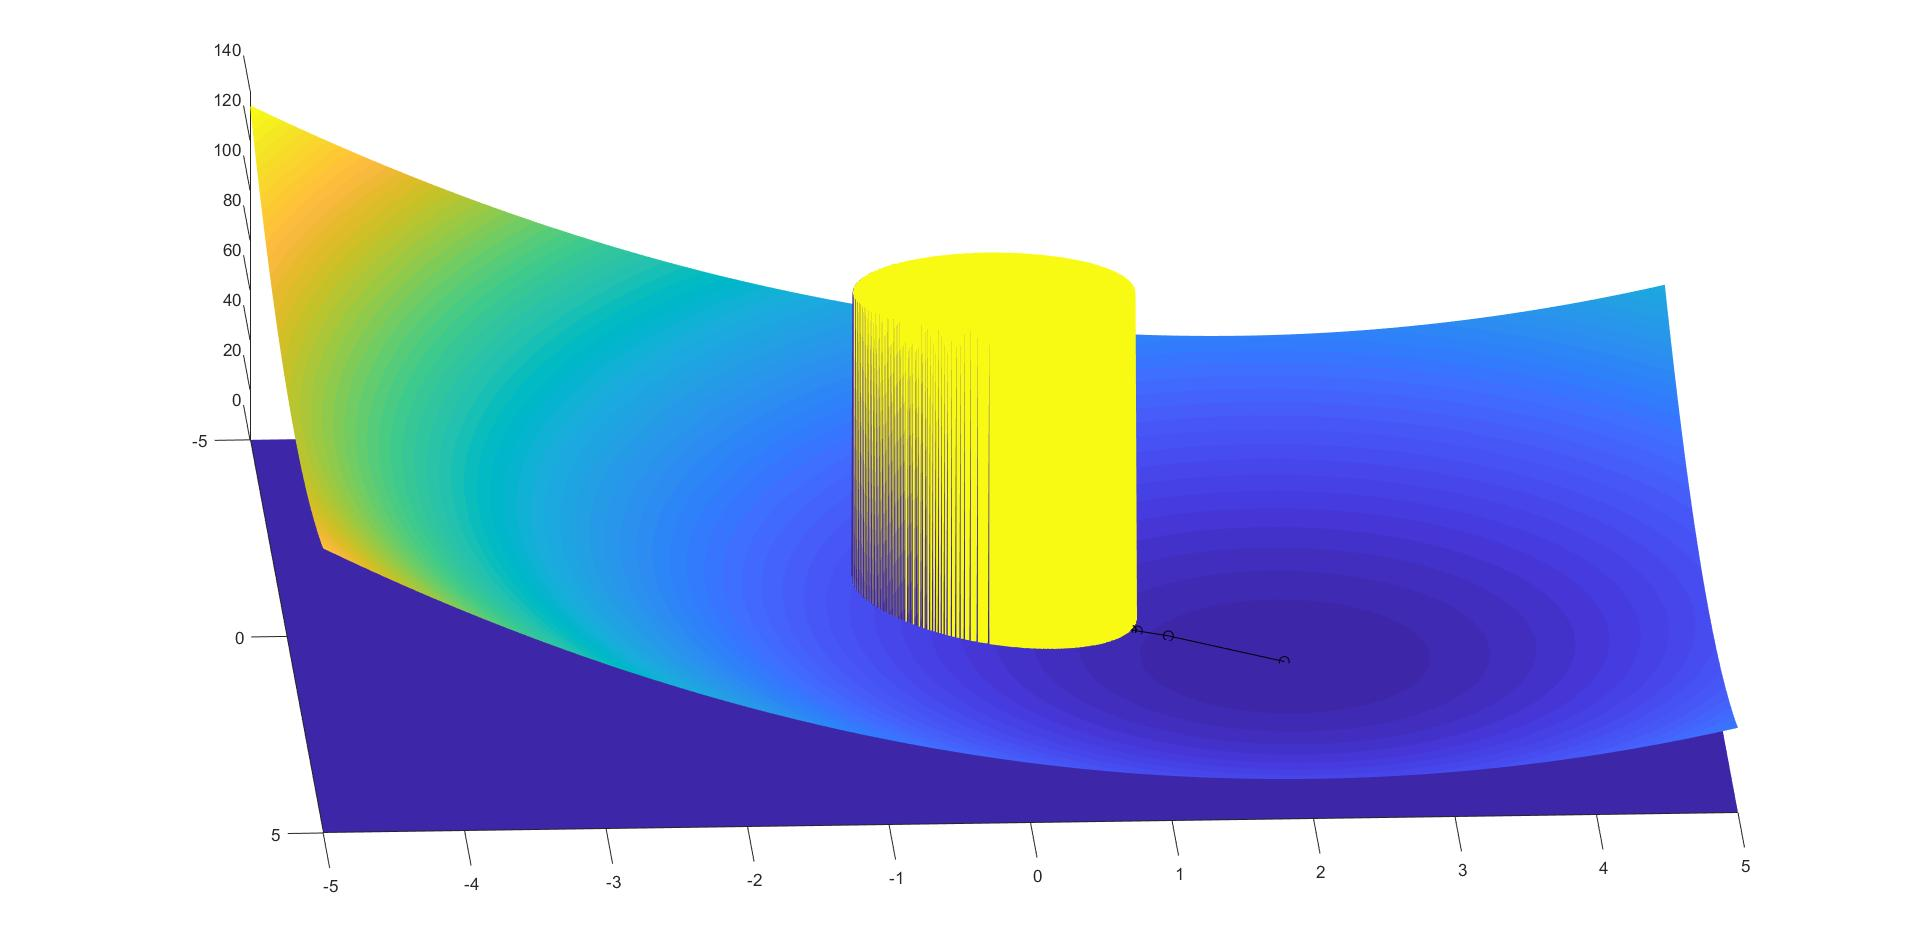
\includegraphics[width=\textwidth]{PenaltyMethod/PenaltyMethod_solved.jpg}
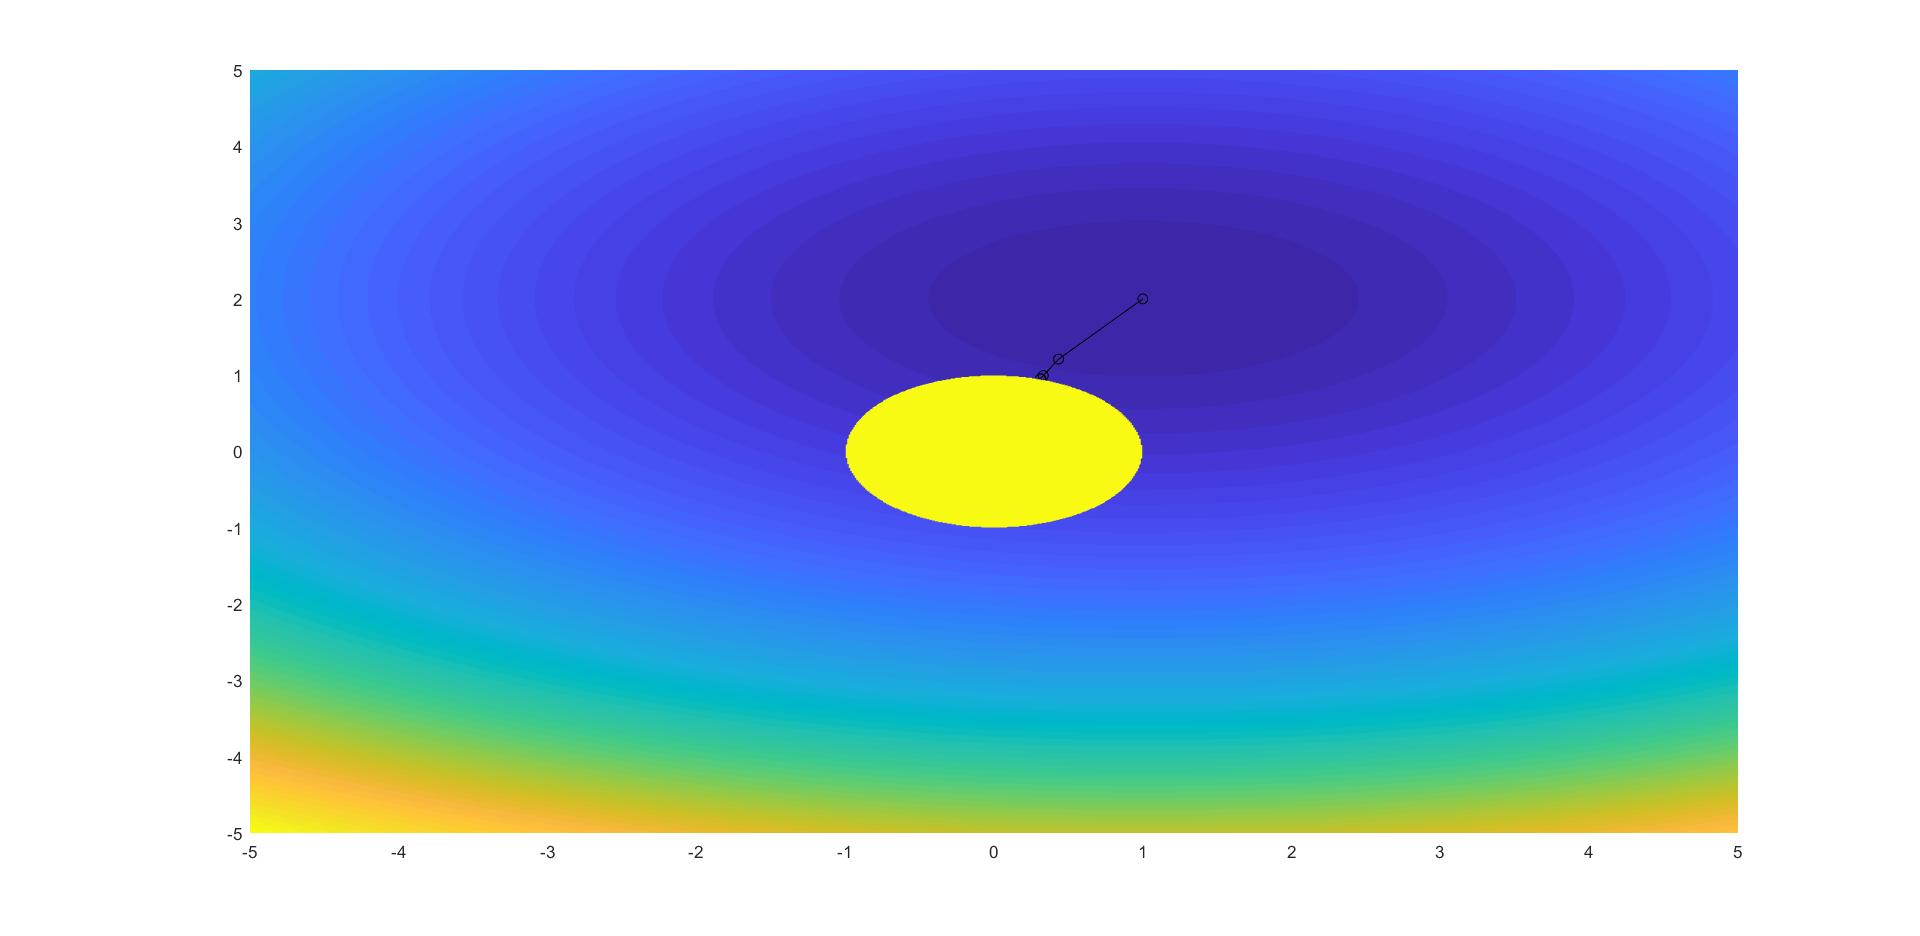
\includegraphics[width=\textwidth]{PenaltyMethod/PenaltyMethod_solved_view(0,90)_.jpg}
\label{fig:solution}
\caption{Objective Function with constraints and penalty method minima points (bottom picture with vertical view on plane $(x_1,x_2)$)}
\end{figure}

\newpage
\section{Conclusions}

 During run program may inform about error:\\
 "...error in GradientDescent.m (line 27) : $\|\nabla*F_p(x_1, x_2, \mu=1250)\| = NaN$".\\
 
 During this case, error pop out for too big value $\mu=1250$ of penalty parameter, from where was found that biggest penalty parameter giving successful run is $\mu=1249$. Also for $\mu=1249$ solution gives best result reaching boundary of valid domain with smallest deviation compared to smaller values of penalty parameter. With smaller values of penalty parameter, points received from gradient descent do not reach valid domain boundary (or reach with deviation). Bigger value of penalty parameter gives smaller deviation, so one may conclude that it is always desired to find value of penalty parameter as big as possible. \\

\end{document}